\documentclass[ST]{subfiles}

\begin{document}
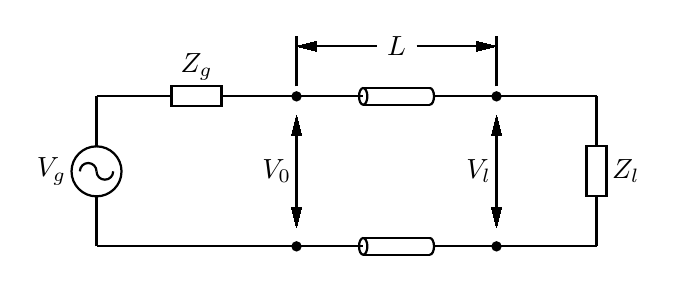
\begin{tikzpicture}[scale=2.54]
% dpic version 2010.11.28 option -g for TikZ and PGF 1.01
\ifx\dpiclw\undefined\newdimen\dpiclw\fi
\global\def\dpicdraw{\draw[line width=\dpiclw]}
\global\def\dpicstop{;}
\dpiclw=0.8bp
\dpiclw=0.8bp
\dpicdraw (0,0)
 --(0,0.25)\dpicstop
\dpicdraw (0,0.375) circle (0.049213in)\dpicstop
\dpicdraw (-0.083333,0.375)
 ..controls (-0.083333,0.398012) and (-0.064679,0.416667)
 ..(-0.041667,0.416667)
 ..controls (-0.018655,0.416667) and (0,0.398012)
 ..(0,0.375)\dpicstop
\dpicdraw (0,0.375)
 ..controls (0,0.351988) and (0.018655,0.333333)
 ..(0.041667,0.333333)
 ..controls (0.064679,0.333333) and (0.083333,0.351988)
 ..(0.083333,0.375)\dpicstop
\dpicdraw (0,0.5)
 --(0,0.75)\dpicstop
\draw (-0.125,0.375) node[left=-1.5bp]{$ V_g$};
\dpicdraw (0,0.75)
 --(0.375,0.75)\dpicstop
\dpicdraw (0.625,0.75)
 --(0.625,0.8)
 --(0.375,0.8)
 --(0.375,0.7)
 --(0.625,0.7)
 --(0.625,0.75)\dpicstop
\dpicdraw (0.625,0.75)
 --(1,0.75)\dpicstop
\draw (0.5,0.8) node[above=-1.5bp]{$ Z_g$};
\dpicdraw[fill=black](1,0.75) circle (0.007874in)\dpicstop
\dpicdraw[fill=black](1,0) circle (0.007874in)\dpicstop
\filldraw[line width=0bp](1.025,0.55625)
 --(1,0.65625)
 --(0.975,0.55625) --cycle
\dpicstop
\dpicdraw (1,0.633344)
 --(1,0.19375)\dpicstop
\filldraw[line width=0bp](0.975,0.19375)
 --(1,0.09375)
 --(1.025,0.19375) --cycle
\dpicstop
\draw (1,0.375) node[left=-1.5bp]{$V_0$};
\dpicdraw (1.6875,0.75)
 --(2,0.75)\dpicstop
\dpicdraw (1,0.75)
 --(1.333333,0.75)\dpicstop
\dpicdraw (1.333333,0.708333)
 --(1.666667,0.708333)\dpicstop
\dpicdraw (1.666667,0.708333)
 ..controls (1.678173,0.708333) and (1.6875,0.726988)
 ..(1.6875,0.75)
 ..controls (1.6875,0.773013) and (1.678173,0.791667)
 ..(1.666667,0.791667)\dpicstop
\dpicdraw (1.666667,0.791667)
 --(1.333333,0.791667)\dpicstop
\dpicdraw (1.333333,0.791667)
 ..controls (1.321827,0.791667) and (1.3125,0.773013)
 ..(1.3125,0.75)
 ..controls (1.3125,0.726988) and (1.321827,0.708333)
 ..(1.333333,0.708333)
 ..controls (1.34484,0.708333) and (1.354167,0.726988)
 ..(1.354167,0.75)
 ..controls (1.354167,0.773013) and (1.34484,0.791667)
 ..(1.333333,0.791667)\dpicstop
\dpicdraw[fill=black](2,0.75) circle (0.007874in)\dpicstop
\dpicdraw[fill=black](2,0) circle (0.007874in)\dpicstop
\filldraw[line width=0bp](2.025,0.55625)
 --(2,0.65625)
 --(1.975,0.55625) --cycle
\dpicstop
\dpicdraw (2,0.633344)
 --(2,0.19375)\dpicstop
\filldraw[line width=0bp](1.975,0.19375)
 --(2,0.09375)
 --(2.025,0.19375) --cycle
\dpicstop
\draw (2,0.375) node[left=-1.5bp]{$V_l$};
\dpicdraw (2,0.75)
 --(2.5,0.75)\dpicstop
\dpicdraw (2.5,0.75)
 --(2.5,0.5)\dpicstop
\dpicdraw (2.5,0.25)
 --(2.55,0.25)
 --(2.55,0.5)
 --(2.45,0.5)
 --(2.45,0.25)
 --(2.5,0.25)\dpicstop
\dpicdraw (2.5,0.25)
 --(2.5,0)\dpicstop
\draw (2.55,0.375) node[right=-1.5bp]{$ Z_l$};
\dpicdraw (2.5,0)
 --(2,0)\dpicstop
\dpicdraw (1.6875,0)
 --(2,0)\dpicstop
\dpicdraw (1,0)
 --(1.333333,0)\dpicstop
\dpicdraw (1.333333,-0.041667)
 --(1.666667,-0.041667)\dpicstop
\dpicdraw (1.666667,-0.041667)
 ..controls (1.678173,-0.041667) and (1.6875,-0.023013)
 ..(1.6875,0)
 ..controls (1.6875,0.023013) and (1.678173,0.041667)
 ..(1.666667,0.041667)\dpicstop
\dpicdraw (1.666667,0.041667)
 --(1.333333,0.041667)\dpicstop
\dpicdraw (1.333333,0.041667)
 ..controls (1.321827,0.041667) and (1.3125,0.023013)
 ..(1.3125,0)
 ..controls (1.3125,-0.023013) and (1.321827,-0.041667)
 ..(1.333333,-0.041667)
 ..controls (1.34484,-0.041667) and (1.354167,-0.023013)
 ..(1.354167,0)
 ..controls (1.354167,0.023013) and (1.34484,0.041667)
 ..(1.333333,0.041667)\dpicstop
\dpicdraw (1,0)
 --(0,0)\dpicstop
\dpicdraw (1,0.8)
 --(1,1.05)\dpicstop
\dpicdraw (2,0.8)
 --(2,1.05)\dpicstop
\filldraw[line width=0bp](1.1,1.025)
 --(1,1)
 --(1.1,0.975) --cycle
\dpicstop
\dpicdraw (1.022906,1)
 --(1.4,1)\dpicstop
\dpicdraw (1.6,1)
 --(1.9,1)\dpicstop
\filldraw[line width=0bp](1.9,0.975)
 --(2,1)
 --(1.9,1.025) --cycle
\dpicstop
\draw (1.5,1) node{$L$};
\end{tikzpicture}
\end{document}

